\documentclass[a4paper,12pt]{article}
\usepackage[utf8]{inputenc}
\usepackage[french]{babel}
\usepackage[T1]{fontenc}
\usepackage[top=2cm,bottom=2cm,left=2cm,right=2cm]{geometry}
\usepackage{graphicx}
\usepackage{wrapfig}
\usepackage{url}

\begin{document}

\begin{titlepage}
	\begin{center}
		\Large{Année universitaire 2016-2017}\\
		\Large{Université de Caen Basse-Normandie}\\[1cm]
		
		\huge{Rapport sur le traitement des projets dans notre IDE}\\
		\vspace{3cm}
		
		Alexis Carreau
		
	\normalsize{\textit{ ~ L2 Informatique}}\\
		\medskip
		\vspace{2cm}
		
	\begin{figure}[h!]
			\begin{center}
				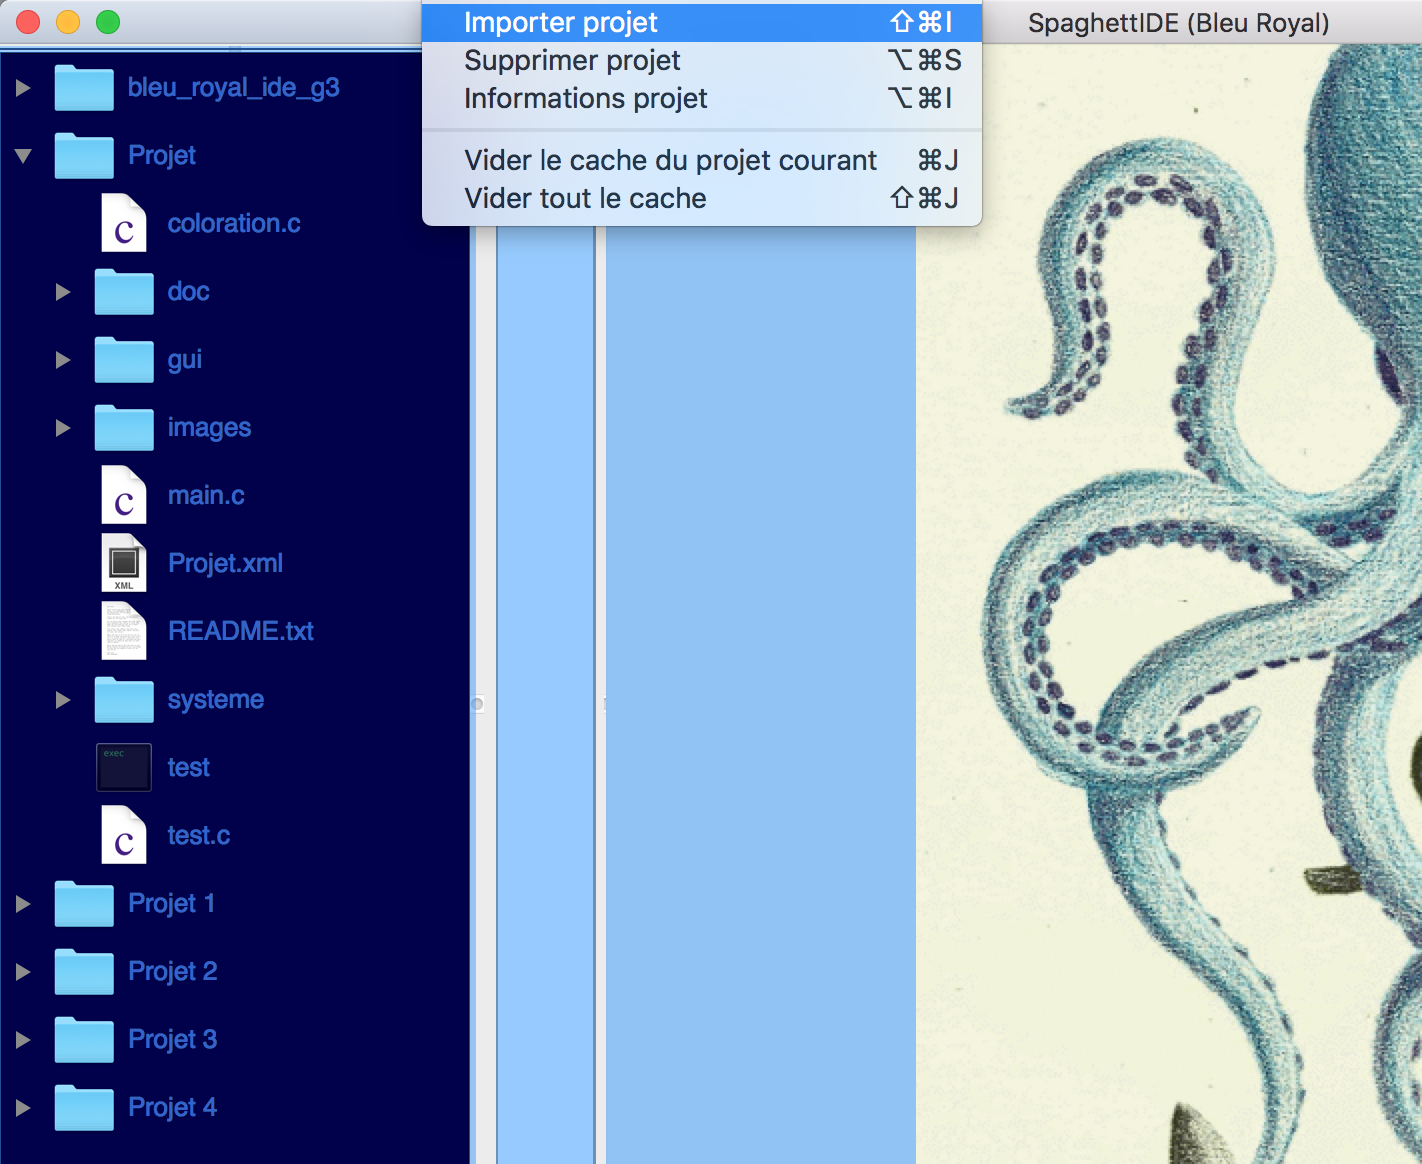
\includegraphics[scale=0.6]{images/project.png}
				\caption{Présentation des projets}
			\end{center}
		\end{figure}
				
	\end{center}
\end{titlepage}

\tableofcontents
\newpage

\section{La mise en place du concept de projet}

Le concept, le principe de projet dans IDE consiste à avoir un dossier Workplace qui comporte tous les dossiers de projet et ce dossier Workplace peut être placé où on veut. Après avoir réalisé ce concept, il ne restait plus qu'à faire les différentes fonctions associées aux projets, comme la création d'un nouveau projet, l'import, la suppression et les informations de chaque projet.
	
\section{La création d'un nouveau projet}
		
Pour créer un nouveau projet, il suffit de cliquer sur le bouton du menu "Nouveau projet", une fenêtre s'ouvre et propose de choisir un nom de projet et un langage et après validation le dossier de projet est créé avec l'xml contenant ses informations dedans. Le dossier est considéré comme un projet et est stocké dans le fichier xml contenant tous les projets.

\begin{figure}[h!]
			\begin{center}
				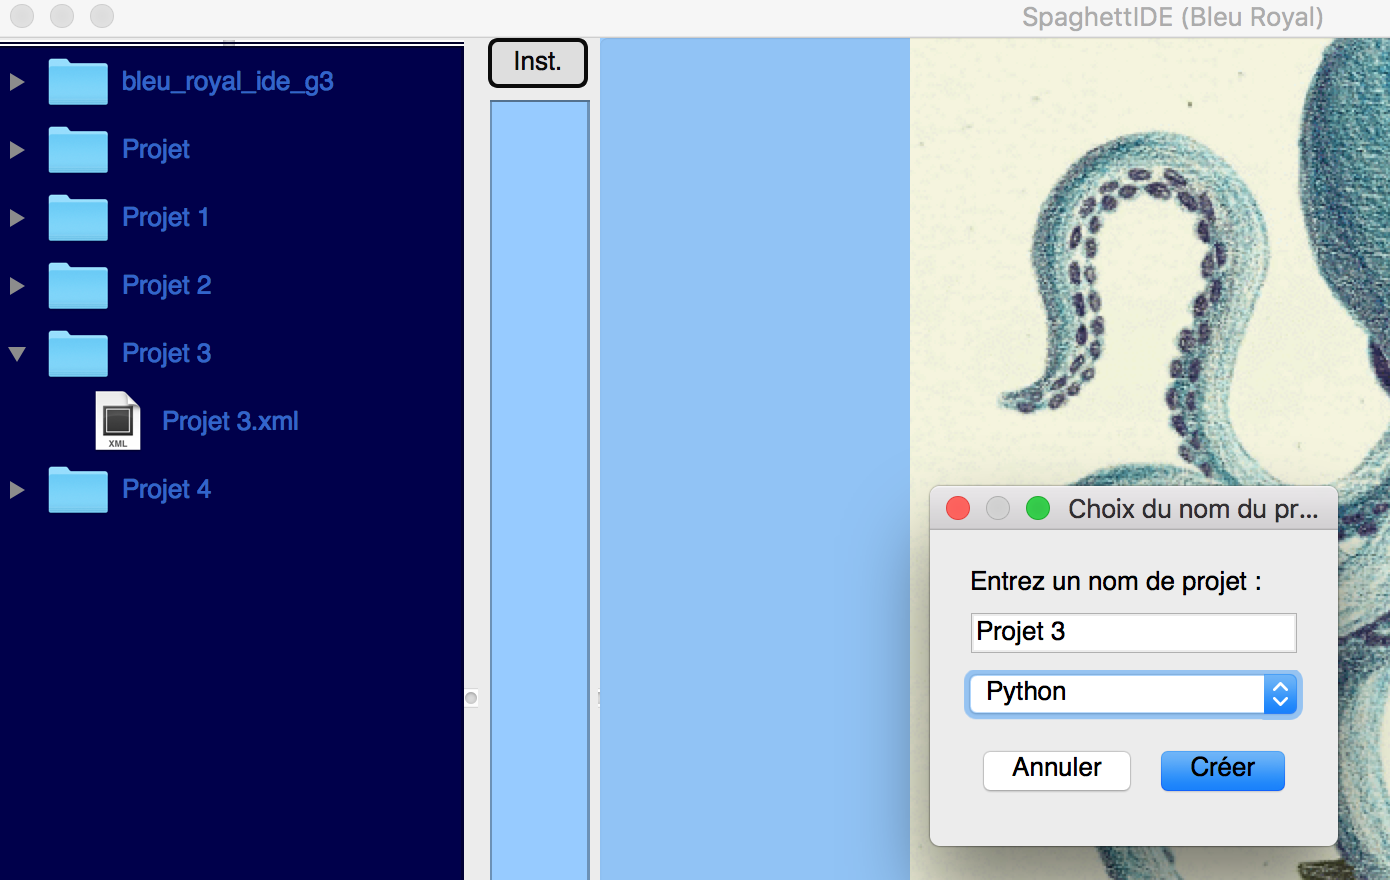
\includegraphics[scale=0.6]{images/creation_project.png}
				\caption{Interface graphique de création de projet}
			\end{center}
		\end{figure}

Nous pouvons maintenant ajouter du code et donc des fichiers dans le nouveau projet créé.

\section{Importation de projet}

Pour importer un projet, un ancien projet en fait, dans le Workplace ou ailleurs, qui ne comprend donc pas de fichier xml, qui n'est donc pas considéré comme un projet encore par l'IDE, il suffit de cliquer sur le bouton du menu "Importer projet". Il l'ajoute au Workplace avec un fichier xml et fait toutes les formalités comme lors de la création d'un projet. Tous les cas sont gérés, à savoir par exemple, l'ajout d'un projet déjà existant, le projet n'est pas écrasé mais rien ne se passe. Il est également possible d'importer un ancien projet qui est dans le Workplace avec le menu clic droit du navigateur de projets et en cliquant sur "Importer le projet".

\begin{figure}[h!]
			\begin{center}
				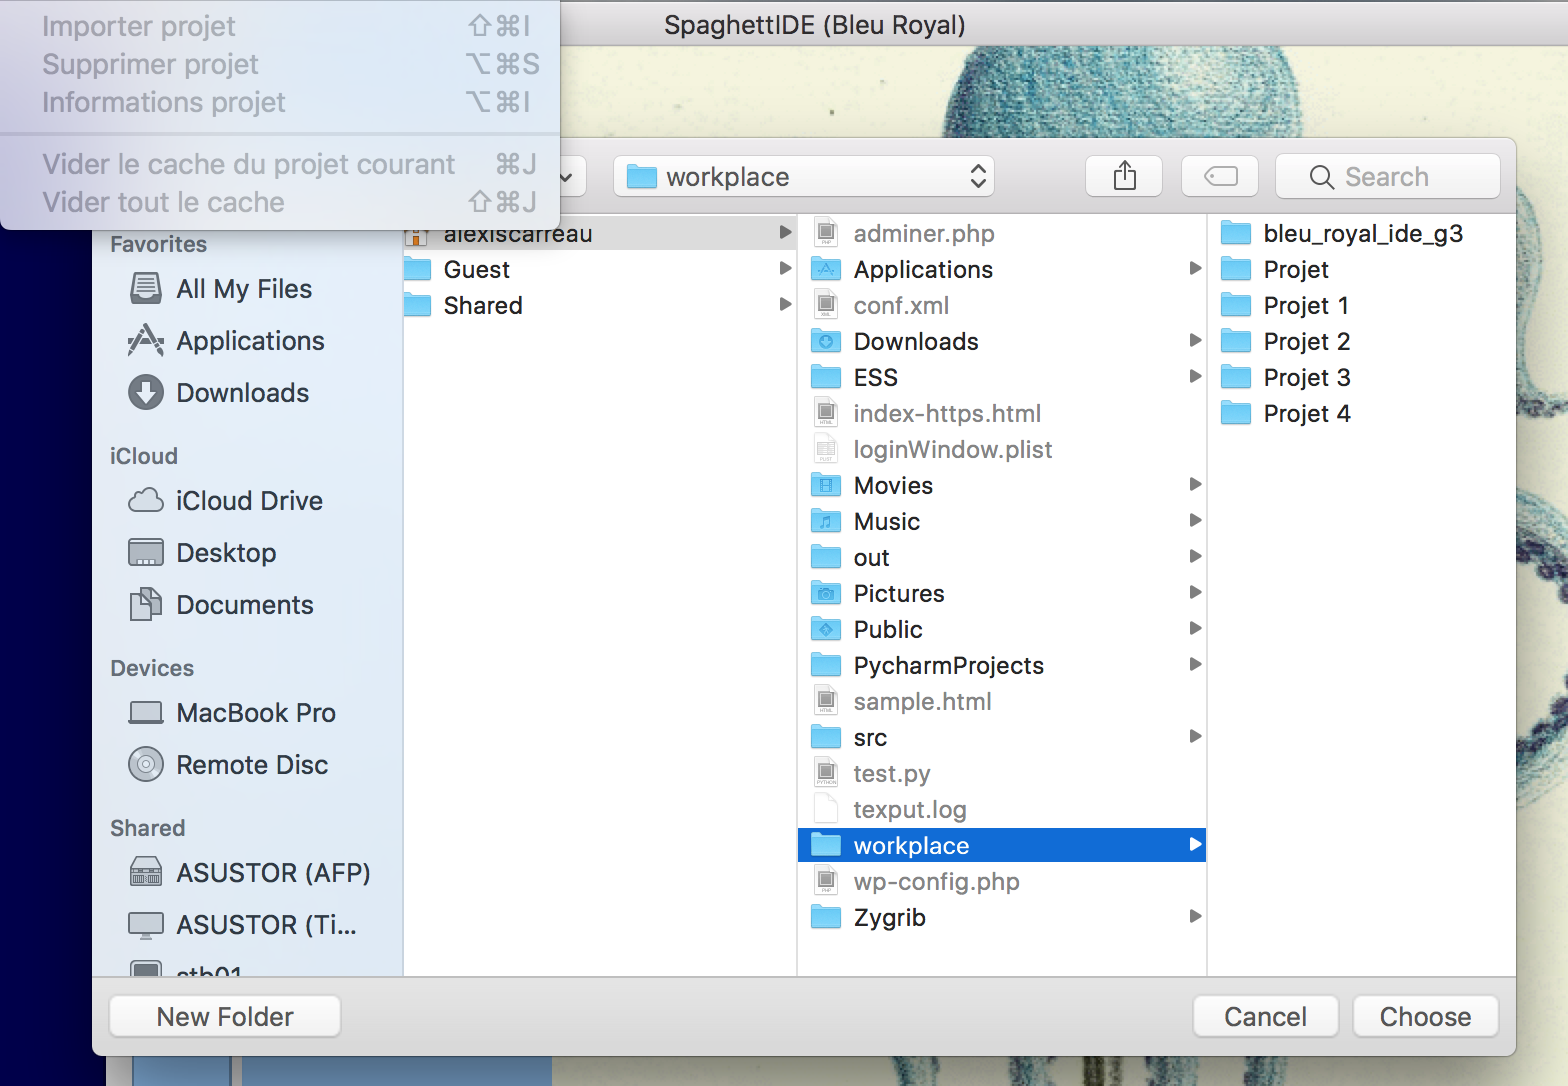
\includegraphics[scale=0.5]{images/import.png}
				\caption{Interface graphique d'import de projet}
			\end{center}
		\end{figure}
		
\section{Suppression de projet}

Pour supprimer un projet, il suffit de cliquer sur le bouton du menu "Supprimer projet". Ainsi, le dossier projet est supprimé du Workplace, nous avons utilisé la commande "shutil.rmtree". Avec la même méthode, nous pouvons supprimer un fichier et même un dossier dans un projet, via par contre le menu clic droit du navigateur de projets, dont nous allons parler dans une prochaine partie.

\begin{figure}[h!]
			\begin{center}
				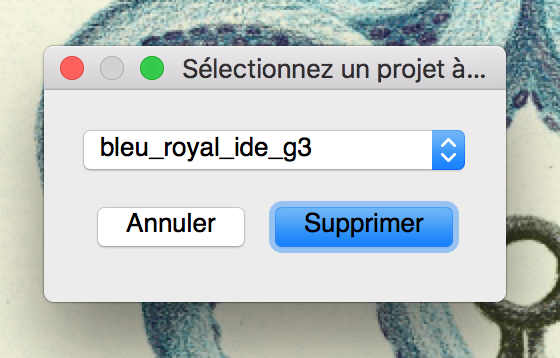
\includegraphics[scale=0.5]{images/supp_project.png}
				\caption{Interface graphique de suppression de projet}
			\end{center}
		\end{figure}

\section{Informations de projet}

Pour accéder aux informations de projet, il suffit de cliquer sur le bouton du menu "Informations projet". Ainsi, une fenêtre s'ouvre et propose de choisir un projet. Une fois le projet choisi, ses informations sont affichées, soit le nom, le langage, la localisation, la date de création et le nombre de fichiers du projet. On peut également modifier les informations, enfin seulement le nom et le langage du projet, pour finir il faut simplement appliquer les modifications effectuées avec le bouton correspondant. Vous pouvez le voir avec les images ci-dessous :

\begin{figure}[h!]
			\begin{center}
				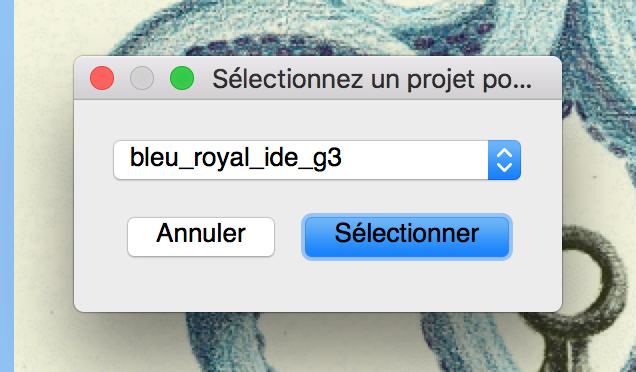
\includegraphics[scale=0.5]{images/info_project1.png}
				\caption{Interface graphique de sélection d'informations de projet}
			\end{center}
		\end{figure}
		
\begin{figure}[h!]
			\begin{center}
				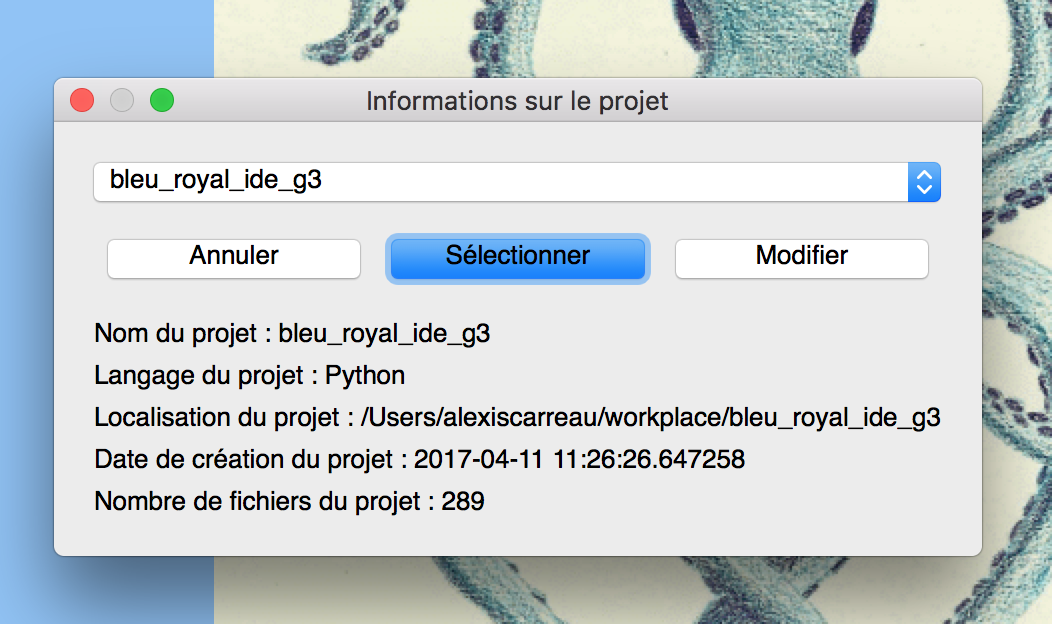
\includegraphics[scale=0.5]{images/info_project2.png}
				\caption{Interface graphique des informations de projet}
			\end{center}
		\end{figure}
		
\begin{figure}[h!]
			\begin{center}
				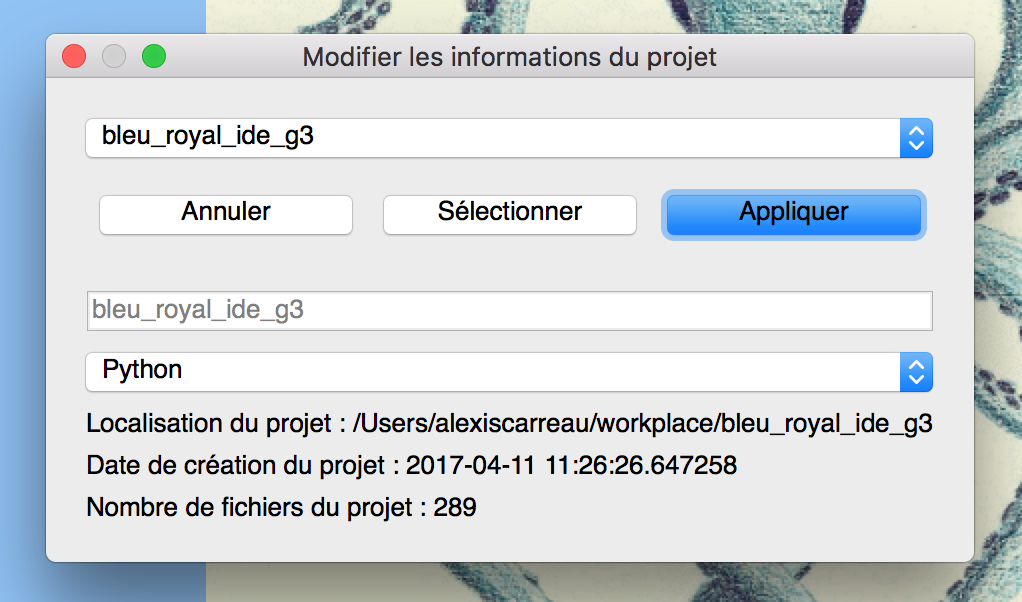
\includegraphics[scale=0.5]{images/info_project3.png}
				\caption{Interface graphique de modification des informations de projet}
			\end{center}
		\end{figure}

\section{Menu clic droit du navigateur de projets}

Un menu s'affichant par un clic droit dans le navigateur de projets a été mis en place permettant d'importer un projet, de le supprimer et d'afficher ses informations. Il est également possible de renommer et de supprimer les dossiers et fichiers présents un projet. C'est donc les mêmes fonctionnalités que précédemment (avec en plus la suppression et la possibilité de renommer les dossiers et fichiers de projets) mais présentées de façon plus pratique, efficace, optimale pour travailler. Vous pouvez le voir avec les images ci-dessous :

\newpage

\begin{figure}[h!]
			\begin{center}
				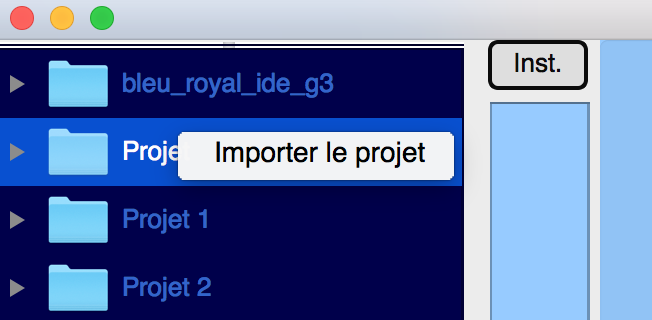
\includegraphics[scale=0.5]{images/right_click_import.png}
				\caption{Import projet via le menu clic droit}
			\end{center}
		\end{figure}
		
\begin{figure}[h!]
			\begin{center}
				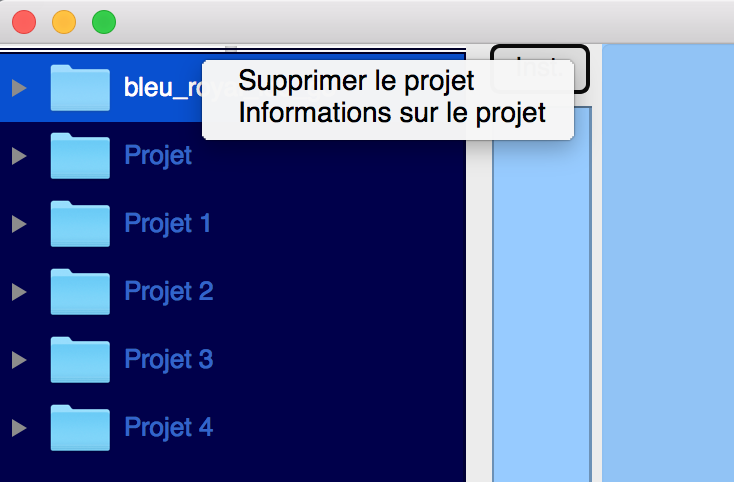
\includegraphics[scale=0.5]{images/right_click_project.png}
				\caption{Suppression et informations de projet via le menu clic droit}
			\end{center}
		\end{figure}
		
\begin{figure}[h!]
			\begin{center}
				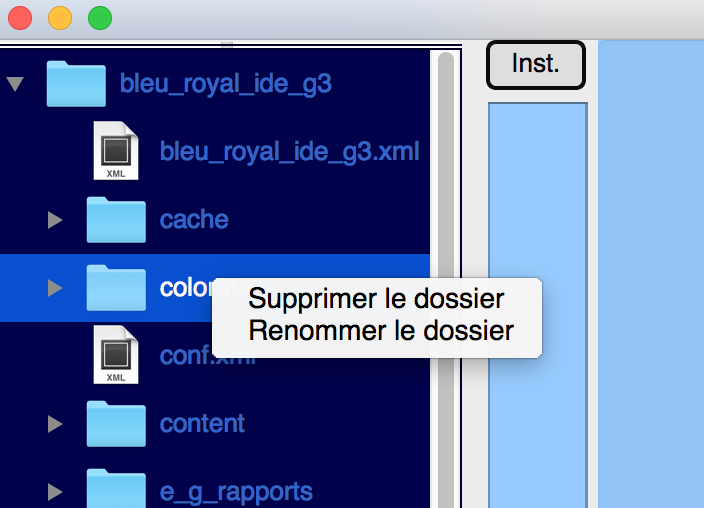
\includegraphics[scale=0.5]{images/right-click-dir.png}
				\caption{Suppression et possibilité de renommer un dossier}
			\end{center}
		\end{figure}
		
\begin{figure}[h!]
			\begin{center}
				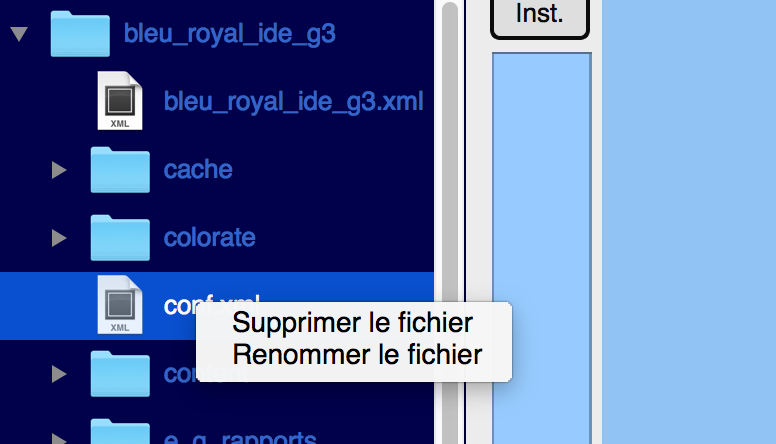
\includegraphics[scale=0.5]{images/right_click_file.png}
				\caption{Suppression et possibilité de renommer un fichier}
			\end{center}
		\end{figure}
		
Lorsque que l'on clique sur le bouton pour renommer, nous obtenons l'affichage d'une fenêtre proposant d'écrire un nouveau nom :

\begin{figure}[h!]
			\begin{center}
				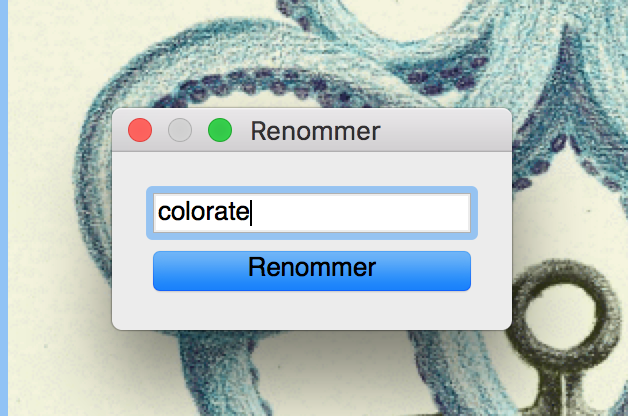
\includegraphics[scale=0.5]{images/rename.png}
				\caption{Renommer un dossier ou un fichier de projet}
			\end{center}
		\end{figure}
		
Lorsque l'on clique sur le bouton pour afficher les informations de projet, nous obtenons un affichage différents de cette même fonctionnalité présentée dans la partie précédente étant donné qu'il faut présenter les informations d'un seul projet. Il est impossible de modifier les informations de part ce menu clic droit, ni de renommer le nom de projet, il faut pour cela faire comme expliqué dans la partie précédente via le menu principal. Nous pouvons le voir avec l'image ci-dessous :

 \begin{figure}[h!]
			\begin{center}
				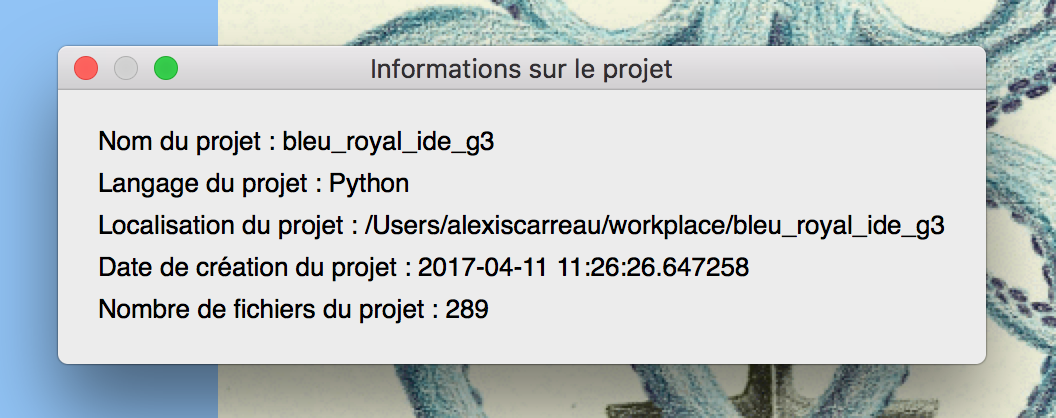
\includegraphics[scale=0.5]{images/info_project4.png}
				\caption{Rendu des informations de projet via le menu clic droit}
			\end{center}
		\end{figure}

\section{Conclusion}

En conclusion, nous pouvons dire que beaucoup de fonctionnalités permettent le traitement des projets confortablement dans notre IDE. La création, l'import, la suppression et les informations de projet sont par exemple des fonctionnalités faciles d'utilisation. Elles sont disponibles dans le menu principal mais également dans le menu clic droit du navigateur de projets. En amélioration, on pourrait imaginer par exemple l'ajout de fonctionnalités, notamment dans le menu clic droit, avec par exemple la possibilité de déplacer un dossier, un fichier de projet dans un autre projet ou directement un projet. Cette fonctionnalité pourrait être faite soit via un bouton dans le menu clic droit, soit directement, de façon standard, en déplaçant avec le curseur de la souris.
		
\end{document}